\documentclass{beamer}
\usetheme{afm}

\title{Risk Measurements}
\author{Matteo Sani - \href{mailto:matteo.sani@unisi.it}{matteo.sani@unisi.it}}

\begin{document}
\begin{frame}[plain]
	\maketitle
\end{frame}

\begin{frame}{VaR and Expected Shortfall}
  \begin{itemize}
  \item Main challenges in quantitative finance: risk measurement and assessment.
  \item There is a wide range of risk measures that spread through the Market, we will concentrate specifically on: Value at Risk (VaR) and Rxpected Shortfall (ES).
  \end{itemize}
  \begin{block}{VaR}
    Value-at-risk is defined as the loss level that will not be exceeded with a certain confidence level during a certain period of time.
    \begin{equation*}
      \textrm{VaR}_{\alpha}(X) = -F^{-1}_X(\alpha)
    \end{equation*}
It is the loss corresponding to the $(100-\alpha)\textrm{th}$ percentile of the portfolio returns over the next $N$ days and by definition it is a function of two parameters: the time horizon (i.e. $N$ days usually set to 1) and the confidence level (usually 95\%). 

VaR asks the question "how bad can things get ?"
\end{block}
\end{frame}

\begin{frame}{Value-at-Risk}
  \begin{figure}[h]
    \begin{center}
      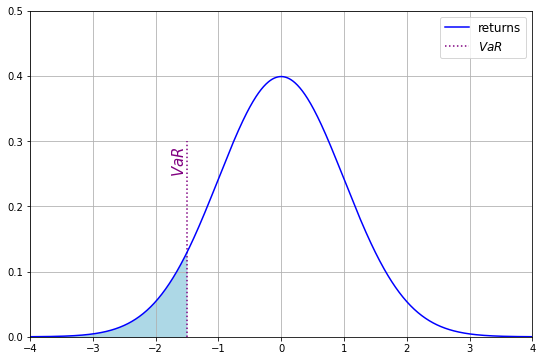
\includegraphics[width=0.5\linewidth]{95_var}
    \end{center}
  \end{figure}
  For example, if a bank's 10-day 99\% VaR is 3 million, it is considered to be only a 1\% chance that losses will exceed 3 million in 10 days. 
\end{frame}

\begin{frame}{Value-at-Risk Drawbacks}
  \begin{itemize}
  \item If VaR is used to limit the risks taken by a trader, it can lead to undesirable results.
  \item A trader is asked that the one-day 99\% VaR of its portfolio must be kept less than 10 million. She could construct a portfolio where there is a 99\% chance that the daily loss is less than 10 million and a 1\% chance that it is 500 million. The trader is satisfying the risk limits imposed by the bank, but is clearly taking unacceptable risks.
  \end{itemize}
  \begin{figure}[h]
    \begin{center}
      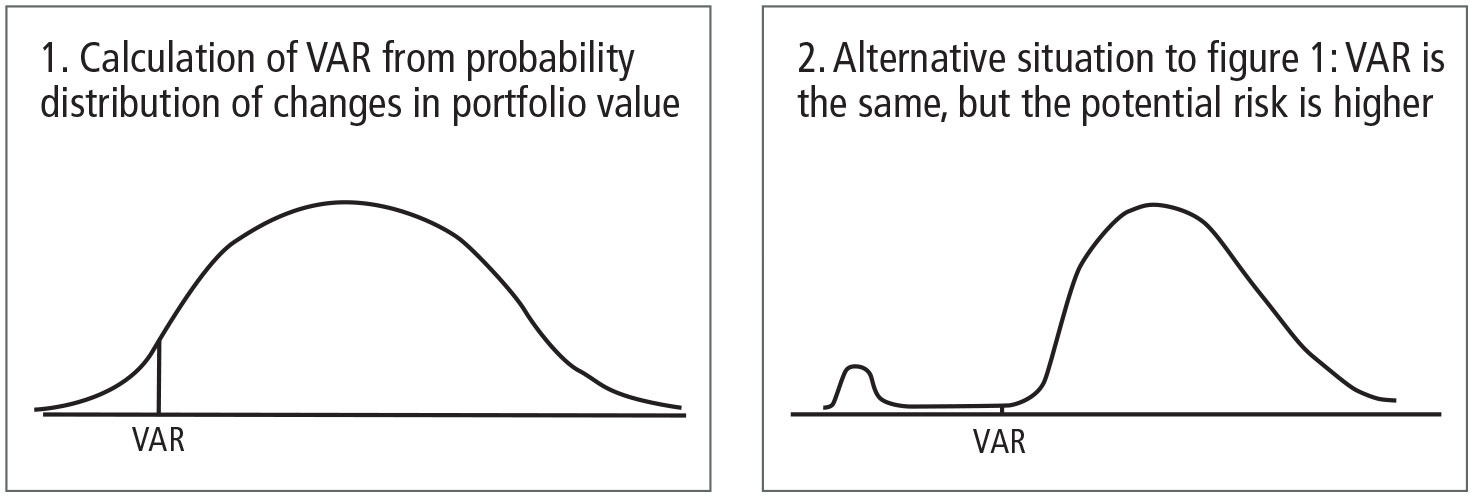
\includegraphics[width=0.7\linewidth]{var_badvar}
    \end{center}
  \end{figure}
\end{frame}

\begin{frame}{Better Definition}
  A measure that produces better incentives for traders is \emph{expected shortfall}.
  \begin{block}{Expected Shortfall}
    A measure that produces better incentives for traders is \emph{expected shortfall}. It is the expected loss during an N-day period, conditional that the loss is greater than the $\alpha^{th}$ percentile of the loss distribution
    \begin{equation*}
      \textrm{ES}_{\alpha}(X) = \frac{1}{\alpha}\int_0^\alpha \textrm{VarR}_p(X) dp
    \end{equation*}
It is the average amount that is lost over a 10-day period, assuming that the loss is greater than the corresponding VaR.

Expected Shortfall asks "if things do get bad, what is our expected loss ?"
\end{block}
\end{frame}

\begin{frame}{Expected Shortfall}
  \begin{figure}[h]
    \begin{center}
      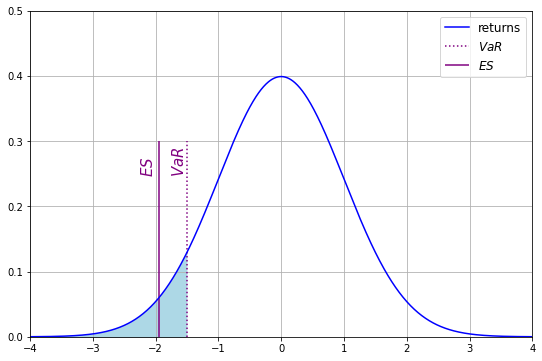
\includegraphics[width=0.5\linewidth]{es}
    \end{center}
  \end{figure}
\end{frame}

\begin{frame}[fragile]{How to "Integrate" in \texttt{python}}
  Numerical integration can be done using \texttt{scipy.integrate.quad} function. Imagine to have to compute
  \begin{equation*}
    \int_{0}^{7} x^2 dx = \frac{x^3}{3}\bigg|_0^7 = 114.33
  \end{equation*}
  \begin{ipython}
from scipy.integrate import quad

def f(x):
  return x**2

print (quad(f, 0, 7))   
\end{ipython}
  \begin{ioutput}
(114.33333333333334, 1.2693549914880957e-12)
\end{ioutput}
Since it is a numerical calculation the first number is the result while the second is the associated uncertainty. 
\end{frame}

\begin{frame}{Parametric Estimate}
  \begin{itemize}
  \item VaR and ES can be estimated essentially in two ways.
  \item \textbf{Parametric}: fit the return historical series of the portfolio and directly apply on the resulting distribution the corresponding definitions of VaR or ES.
    \begin{columns}
      \column{0.5\linewidth}
      Many theories in finance assume the normality of stock returns, unfortunately normality is not a realistic assumption as can be seen by performing a Gaussian fit to the return distribution.
      
      A better model results in a more precise estimate of VaR and ES can be obtained with a t-student.
      \column{0.5\linewidth}
      \begin{figure}[h]
        \begin{center}
          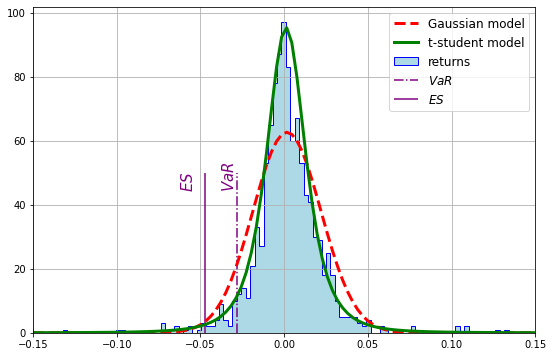
\includegraphics[width=0.9\linewidth]{parametric_var}
        \end{center}
      \end{figure}
    \end{columns}
  \end{itemize}
\end{frame}

\begin{frame}{Historical Simulation}
  \begin{itemize}
  \item Alternatively we can avoid any assumption on the return distribution, by random sampling on the historical returns directly. 
  \item The parameter estimation is not required in this case, but we heavily rely on the assumption that past behaviors are indicative of what might happen in the future. 
  \item Historical series is needed to be as large as possible otherwise our results will be affected by lack of statistics. 
    VaR and ES can be estimated essentially in two ways.
  \end{itemize}
  \begin{figure}[h]
    \begin{center}
      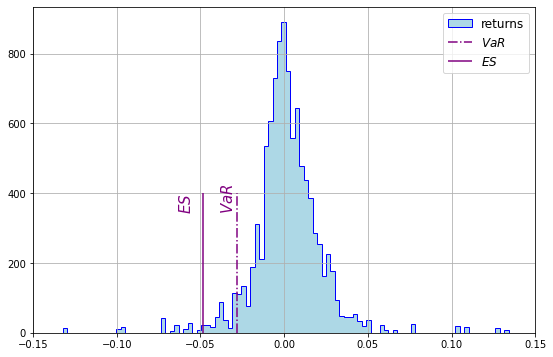
\includegraphics[width=0.4\linewidth]{historical_var}
    \end{center}
  \end{figure}
\end{frame}

\begin{frame}{Stress and Back Testing}
  \begin{itemize}
  \item It is generally useful to check how VaR would behave under the most extreme market moves seen in the last years.
  \item This kind of test is called \emph{stress-test}; it is done by extracting from the historical series particular days with exceptionally large variation of the market variables, to take into account extreme events that can happen more frequently in reality than in a simulation (where usually Gaussian tails are assumed). 
  \item \emph{Backtesting} consists of assessing how well the VaR estimate would have performed in the past. 
  \item Basically it has to be tested how often the daily loss exceeded the daily X\% VaR just computed. 
  \item If it happens on about (100 - X)\% of the times we can be confident that our estimate is correct. 
  \item Clearly back-testing makes sense only if VaR has been estimated on an independent historical sample with respect to that used in the test.
  \end{itemize}
\end{frame}

\begin{frame}{Credit VaR}
  \begin{itemize}	
    \item Credit VaR is defined as a percentile of the \emph{credit loss} distribution. 
    \item In this case we are concerned with the default risk associated to counter-parties instead of the market risk.
    \item The \emph{exposure} $EE(\tau)$ is defined as the sum of the discounted cash flows at the default date $\tau$. 
    \item The corresponding \emph{loss} is then given by $L =(1-R)\cdot EE(\tau)$ where $L$ is non-zero only in scenarios of early counter-party default.
    \item Credit VaR can be expressed as the $\alpha$-quantile of the distribution of $L$ and the Time horizon is usually set to one year and the percentile to the 99.9th (i.e. it returns the loss that is exceeded only in 1 case out of 1000).
  \end{itemize}
\end{frame}
  
\begin{frame}{Credit VaR and MC Simulation}
  \begin{itemize}
    \item Credit VaR can be calculated through a simulation of the evolution of a portfolio up to the risk horizon, including possible defaults of the counter-parties.
    \item In each experiment the portfolio is priced obtaining a number of scenarios to draw the loss distribution.
    \item Consider a portfolio of 20 zero coupon bonds each one with a default probability of 8\% and the same face value (100 EUR). The recovery rate in case of default is 40\% and the risk free rate is 1\%.
    \end{itemize}
\end{frame}

\begin{frame}{CVA}
  \begin{itemize}
  \item Suppose you have a portfolio of derivatives and a counter-party defaults. Two scenarios may happen ($PV$ present value of the portfolio to the surviving party, us, $\tau$ default time)
    \begin{itemize}
    \item $PV_{\textrm{portfolio}}(\tau) > 0$: then you actual gain only the recovery fraction of the value;
    \item $PV_{\textrm{portfolio}}(\tau) < 0$: you have to pay it in full to the liquidators of the defaulted entity.
    \end{itemize}
  \item This undesirible asymmetry can be corrected by changing the definition of the deal value by subtracting a positive adjustment to the risk-less value. This adjustment is called \emph{Credit Valuation Adjustment} (CVA)
\begin{align*}
  \textrm{CVA} &= (1-R)\int_0^{T} D(t)\cdot EE(t) dQ(t) \\
  \textrm{CVA} &= (1-R)\sum_i D(t_i)\cdot EE(t_i)\cdot  Q(t_{i-1}, t_i) \quad \textrm{discrete version}
\end{align*}
where $T$ is the portfolio maturity, $D$ the discount factor, $EE=\mathbb{E}[\max(0, PV_{\textrm{portfolio}})]$ the expected exposure, and $dQ$ the default probability between $t$ and $t + dt$.
  \end{itemize}
\end{frame}

\begin{frame}{DVA}
  \begin{itemize}
  \item \emph{Credit VaR measures the risk of losses faced due to the default of some counter-party, while CVA measures the price adjustment of a contract due to this risk}.
  \item A similar adjustment seen from the point of view of the counter-party is positive, and is called \emph{Debit Valuation Adjustment} (DVA). 
  \item It is positive because the early default of the client itself would imply a discount on its payment obligations, and this means a gain.
  \item When both parties have a non-null probability of default, they consistently include both CVA and DVA into the valuation.
  \item So they will mark \emph{a positive CVA to be subtracted} and \emph{a positive DVA to be added} to the default-risk-free price of the deal. 
  \item The CVA of one party will be the DVA of the other one and vice versa.
    \begin{equation*}
      \textrm{price = default risk free price + DVA - CVA}
    \end{equation*}
  \end{itemize}
\end{frame}

\begin{frame}{CVA Computation}
  \begin{itemize}
  \item CVA can be computed with Monte Carlo simulation
    \begin{enumerate}
    \item compute the portfolio value at each time point for each MC scenario;
    \item calculate the CVA using one of the equation above;
    \item average the CVA of all the scenarios to get its estimate.
    \end{enumerate}
  \item Example: imagine a 3-years zero coupon bond with a face value $FV = 100$. The bond issuer has the following default probabilities 10\%, 20\% and 30\% for 1, 2 and 3 years respectively and the recovery rate is 40\%.  The risk free rate is instead 3\% flat.
  \end{itemize}
\end{frame}

\end{document}

